\documentclass[xcolor=dvipsnames]{beamer}
\makeatletter\def\Hy@xspace@end{}\makeatother 
\usepackage{graphicx, color, amssymb, amsmath, bm, rotating, graphics,
epsfig, multicol, amsthm}
\usepackage[english]{babel}
\usepackage[T1]{fontenc}
\usepackage[ansinew]{inputenc}
\usepackage[authoryear]{natbib}
%\newcommand{\newblock}{}  %needed to make beamer and natbib play nice
\usepackage{tikz}
\usetikzlibrary{fit}					% fitting shapes to coordinates
\usetheme{Boadilla}
\usecolortheme[named=Red]{structure}
\setbeamercovered{transparent}
\beamertemplatenavigationsymbolsempty
\newcommand\ind{\protect\mathpalette{\protect\independenT}{\perp}}
\def\independenT#1#2{\mathrel{\rlap{$#1#2$}\mkern2mu{#1#2}}}
\newcommand\N{\mathcal{N}}
\graphicspath{{../doc/plots/}}
\title[Interweaving MCMC Strats for DLMs]{Interweaving Markov Chain Monte Carlo Strategies for Efficient
Estimation of Dynamic Linear Models}
%\subtitle{}
\author[M. Simpson]{Matthew Simpson}
\date{}
\institute[Deps of Stat \& Econ, ISU]{Departments of Statistics and Economics, Iowa State University}


%\title[short title]{long title}
%\subtitle[short subtitle]{long subtitle}
%\author[short name]{long name}
%\date[short date]{long date}
%\institution[short name]{long name}

% very important to use option [fragile] for frames containing code output!

\begin{document}

\begin{frame}
\titlepage
\begin{center}
with Jarad Niemi and Vivekananda Roy\\~\\
\scriptsize{Department of Statistics, Iowa State University}
\end{center}
\end{frame}

\begin{frame}
\frametitle{Interweaving: A Motivating Example}
Adapted from \citet{yu2011center}, suppose:
\begin{align*}
y|\theta, \phi & \sim \N(\theta, V) \\
\theta|\phi & \sim \N(\phi, W) 
\end{align*}
with $V$, $W$ known and $p(\phi)\propto 1$.\\~\\

DA algorithm based on $\theta$:
\begin{align*}
\theta|\phi,y &\sim \N\left(\frac{V\phi + Wy}{V+W}, \frac{VW}{V+W}\right)\\
\phi |\theta, y &\sim \N(\theta, W)
\end{align*}
\end{frame}

\begin{frame}
\frametitle{Interweaving: A Motivating Example}
Let $\gamma = \theta - \phi$. Then:
\begin{align*}
y|\gamma, \phi & \sim \N(\phi + \gamma, V) \\
\gamma|\phi & \sim \N(0, W) 
\end{align*}
DA algorithm based on $\gamma$:
\begin{align*}
\gamma|\phi,y &\sim \N\left(\frac{W(\phi - y)}{V+W}, \frac{VW}{V+W}\right)\\
\phi |\gamma, y &\sim \N(y-\gamma, V)
\end{align*}
\end{frame}

\begin{frame}
\frametitle{Interweaving: A Motivating Example}
Alternate between two DAs (alternating algorithm):
\begin{align*}
{\color{blue}[\theta|\phi,y]} \to {\color{blue}[\phi|\theta,y]} \to [\gamma|\phi,y] \to [\phi|\gamma,y]
\end{align*}\\~\\
Weave two DAs together (interweaving algorithm):
\begin{align*}
{\color{blue}[\theta|\phi,y]} \to {\color{blue}[\phi|\theta,y]} \to {\color{red}[\gamma|\phi,\theta,y]} \to [\phi|\gamma,y]
\end{align*}\\~\\\pause
The interweaving algorithm obtains {\bf IID} draws from the posterior of $\phi$.
\end{frame}

\begin{frame}
\frametitle{Global Interweaving Strategy (GIS)}
From \citet{yu2011center}: target posterior distribution $p(\phi|y)$ with two DAs $\theta$ and $\gamma$ such that
\begin{align*}
\int p(\theta,\phi|y) d\theta = p(\phi|y) \ \ \ \ \mbox{and}\ \ \ \int p(\gamma,\phi|y) d\gamma = p(\phi|y) 
\end{align*}
Then:
\begin{align*}
[\theta|\phi,y] \to [\gamma|\theta,y] \to [\phi|\gamma,y]
\end{align*}
or more commonly:
\begin{align*}
[\theta|\phi,y] \to [\phi|\theta,y] \to {\color{blue}[\gamma|\phi,\theta,y]} \to [\phi|\gamma,y]
\end{align*}
\end{frame}

\begin{frame}
\frametitle{Ancillary-Sufficiency Interweaving Strategy (ASIS)}
GIS where one DA is a sufficient augmentation (SA) and the other is an ancillary augmentation (AA).\\~\\
\begin{itemize}
\item$\theta$ is an SA if $p(y|\theta,\phi)=p(y|\theta)$ (AKA centered augmentation)\\~\\
\item$\theta$ is an AA if $p(\theta|\phi)=p(\theta)$ (AKA non-centered augmentation)\\~\\
\end{itemize}
Componentwise Interweaving Strategy (CIS):\\~\\
\begin{itemize}
\item Motivation: Finding an SA--AA pair is often difficult for $\phi=(\phi_1,\phi_2)$, but not for $\phi_1$ and $\phi_2$ separately.\\~\\
\item Basic idea: GIS (or ASIS) for sub-blocks of $\phi$.\\~\\
\item Can use the same DA in multiple sub-blocks of $\phi$.
\end{itemize}
\end{frame}

\begin{frame}[fragile]
  \frametitle{The Dynamic Linear Model} 
  For $t=1,2,...,T$
  \begin{align*}
    y_t  =&F_t\theta_t +  v_t  \qquad \mbox{(observation equation)}\\
    \theta_t =& G_t\theta_{t-1} + w_t \qquad \mbox{(system equation)}
  \end{align*} 
  with $v_t\stackrel{iid}{\sim}\N_k(0,V)$ independent of $w_t\stackrel{iid}{\sim}\N_p(0,W)$.\\~\\

\begin{figure}
  \centering
    \tikzstyle{state}=[circle, thick, minimum size=1.2cm, draw=black!80]
    \tikzstyle{obs}=[circle, thick, minimum size=1.2cm, draw=black!80]
  \begin{tikzpicture}[>=latex,text height=1.5ex,text depth=0.25ex]
    \matrix[row sep=0.5cm,column sep=0.5cm]{
    % First line: Observations
    &
    \node (y_t-1) [obs]{$y_{t-1}$}; &
    &
    \node (y_t) [obs]{$y_{t}$}; &
    &
    \node (y_t+1) [obs]{$y_{t+1}$}; &
    \\
    % Second line: States
    \node (theta_t-2) {$\cdots$}; &
    \node (theta_t-1) [state]{$\theta_{t-1}$}; &
    &
    \node (theta_t) [state]{$\theta_{t}$}; &
    &
    \node (theta_t+1) [state]{$\theta_{t+1}$}; &
    \node (theta_t+2) {$\cdots$}; \\
    };
    
    % The diagram elements are now connected through arrows:
    \path[->]
    (theta_t-2) edge (theta_t-1)
    (theta_t-1) edge (theta_t)
    (theta_t) edge (theta_t+1)
    (theta_t+1) edge (theta_t+2)
    (theta_t-1) edge (y_t-1)
    (theta_t) edge (y_t)
    (theta_t+1) edge (y_t+1)
    ;
  \end{tikzpicture}
  \end{figure}

For convenience define $y\equiv(y_1',\cdots,y_T')'$ and $\theta\equiv(\theta_0',\cdots,\theta_T)'$.

\end{frame}

\begin{frame}
  \frametitle{The Dynamic Linear Model} 
Let $\phi$ denote the unknown parameter. Potentially $F_t(\phi)$ and $G_t(\phi)$ but assume they are constant and $\phi=(V,W)$\\~\\

Priors: independently \\~\\
\begin{itemize}
\item[]$\theta_0\sim \N_p(m_0,C_0)$, $V\sim IW(\Lambda_V,\lambda_V)$, and $W\sim IW(\Lambda_W,\lambda_W)$\\~\\
\end{itemize}

Want to apply GIS and ASIS in particular, but suppose $\eta$ is a SA and $p(y,\eta|\phi)$ is Gaussian.\\~
\begin{itemize}
\item[] Then under weak condtions, $p(\phi|\eta,y)$ and $p(\phi|y)$ have a similar form.
\end{itemize}

\end{frame}

\begin{frame}
\frametitle{Data Augmentations for the DLM}
Standard DA: states $\theta$. In terms of $\theta$, the model is:
\begin{align*}
y_t|\theta,V,W \stackrel{ind}{\sim} & \N_k(F_t\theta_t,V)\\ 
\theta_t|\theta_{0:(t-1)},V,W \sim & \N_p(G_t\theta_{t-1},W)
\end{align*} 
{\color{blue}$\theta$ is an SA for $W|V$ and an AA for $V|W$.}\\~\\

Scaled disturbances $\gamma\equiv(\gamma_0',\cdots,\gamma_T)'$ \citep{fruhwirth2004efficient}.
\begin{itemize}
\item[]$\gamma_0=\theta_0$ and $\gamma_t=L_W^{-1}(\theta_t - G_t\theta_{t-1})=L_W^{-1}w_t$ where $L_W$ is the Cholesky decomposition of $W$.
\end{itemize}
Then:
\begin{align*}
y_t|\gamma,V,W \stackrel{ind}{\sim} & \N_k(F_t\theta_t(\gamma,W),V) \\
\gamma_t|V,W \stackrel{iid}{\sim} & \N_p(0,I_p)
\end{align*} 

{\color{blue}$\gamma$ is an AA for $(V,W)$.}

\end{frame}

\begin{frame}
\frametitle{New Data Augmentations for the DLM}
Scaled errors $\psi\equiv(\psi_0',\cdots,\psi_T')'$:
\begin{itemize}
\item[]$\psi_0=\theta_0$ and $\psi_t=L_V^{-1}(y_t - F_t\theta_t)=L_V^{-1}v_t$ where $L_V$ is the Cholesky decomposition of $V$.
\end{itemize}
For convenience, assume $F_t$ is square and invertible for all $t$.\\~
 
In terms of $\psi$ the model is:
\begin{align*}
y_t|\psi,V,W \stackrel{ind}{\sim} &\N_p(\mu_t(\psi,V),F_tWF_t')\\
\psi_t|V,W \stackrel{iid}{\sim} &\N_p(0,I_p)
\end{align*} 
where $\mu_t(\psi,V)$ is complicated.\\~\\

{\color{blue}$\psi$ is an AA for $(V,W)$.}
\end{frame}

\begin{frame}
\frametitle{New Data Augmentations for the DLM}
Wrongly-scaled disturbances $\tilde{\gamma}\equiv(\tilde{\gamma}_0',\cdots,\tilde{\gamma}_T')'$:\\~\\
\begin{itemize}
\item[]$\tilde{\gamma}_0=\theta_0$ and $\tilde{\gamma}_t=L_V^{-1}(\theta_t - G_t\theta_{t-1})=L_V^{-1}w_t$\\~\\
\end{itemize}

Wrongly-scaled errors $\tilde{\psi}\equiv(\tilde{\psi}_0',\cdots,\tilde{\psi}_T')'$:\\~\\
\begin{itemize}
\item[]$\tilde{\psi}_0=\theta_0$ and $\tilde{\psi}_t=L_W^{-1}(y_t - F_t\theta_{t})=L_W^{-1}v_t$\\~\\
\end{itemize}

{\color{blue} $\tilde{\gamma}$ is an SA for $W|V$ and $\tilde{\psi}$ is an SA for $V|W$.}
\end{frame}

\begin{frame}[fragile]
\frametitle{Evaluating the Strategies: the Local Level Model}
Model: for $t=1,2,...,T$
\begin{align*}
    y_t|\theta  \stackrel{ind}{\sim}&\N_1(\theta_t,V) \qquad (\mbox{observation equation})\\
    \theta_t|\theta_{0:(t-1)} \sim& \N_1(\theta_{t-1},W) \qquad (\mbox{system equation})
  \end{align*} 

Let $V^*$ and $W^*$ denote the true values used to simulate the time series.\\~\\

Independent priors:
\begin{itemize}
\item $\theta_0\sim N(0, 10^7)$, $V\sim IG(5, 4V^*)$ and $W\sim IG(5, 4W^*)$.\\~\\
\end{itemize}

Simulation Setup:
\begin{itemize}
\item Simulated data: $T=10$, $T=100$ \& $T=1000$ and $V^*$, $W^*$ $=10^{i/2}$ with $i=-4,-3,\cdots,4$.
\item Each sampler was used to fit the model to each dataset using one Markov chain started at $(V^*,W^*)$.
\end{itemize}


\end{frame}

\begin{frame}
\frametitle{LLM Results --- ESP for T=100}
\centering
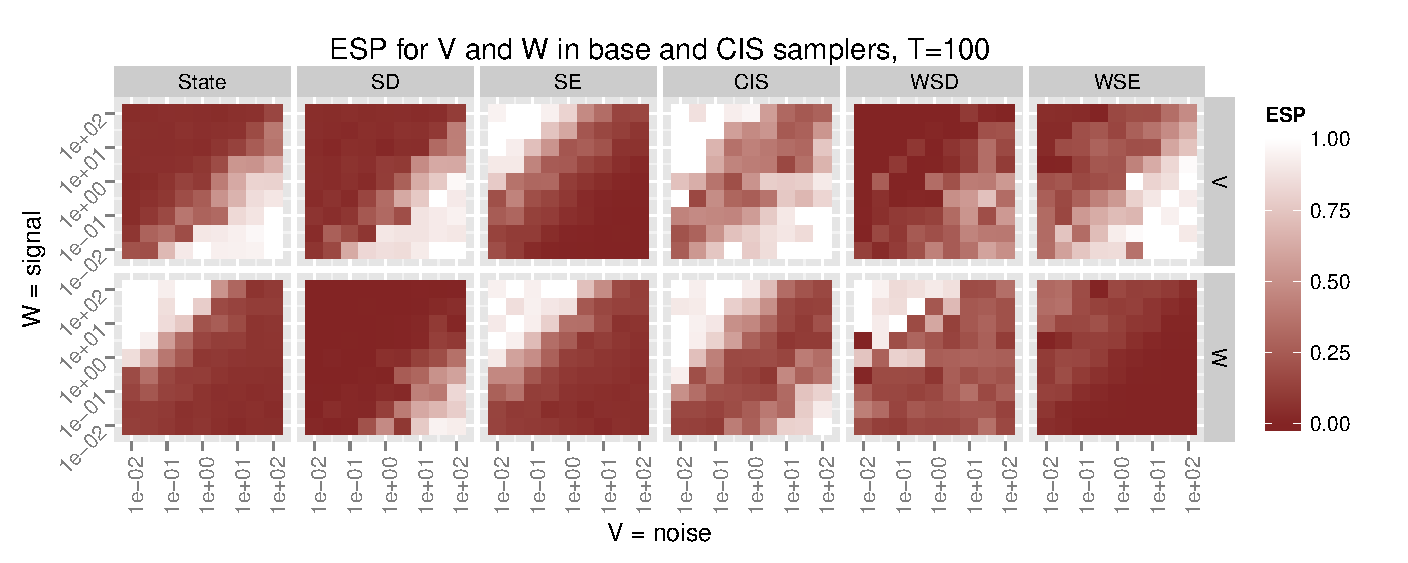
\includegraphics[width=0.59\textwidth]{basecisESplot100}\\
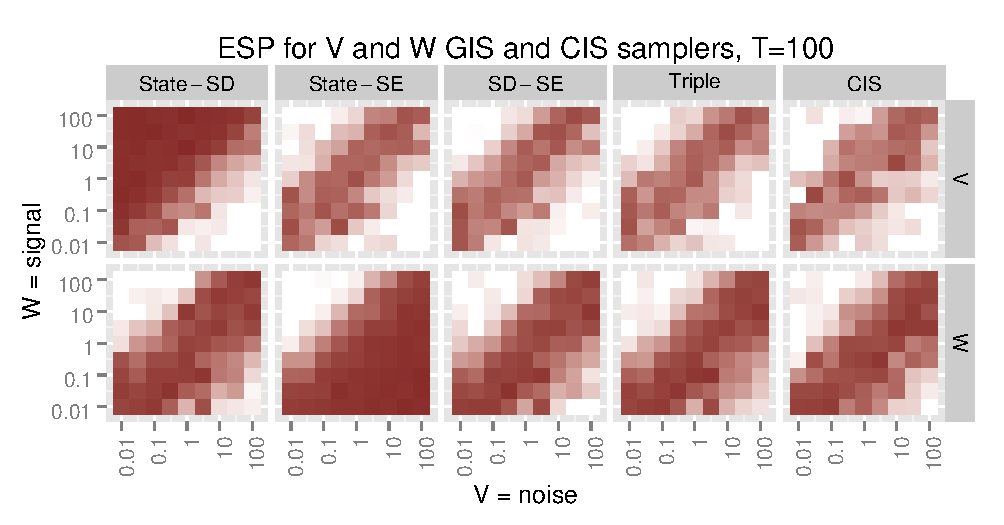
\includegraphics[width=0.53\textwidth]{altintESplotV100}
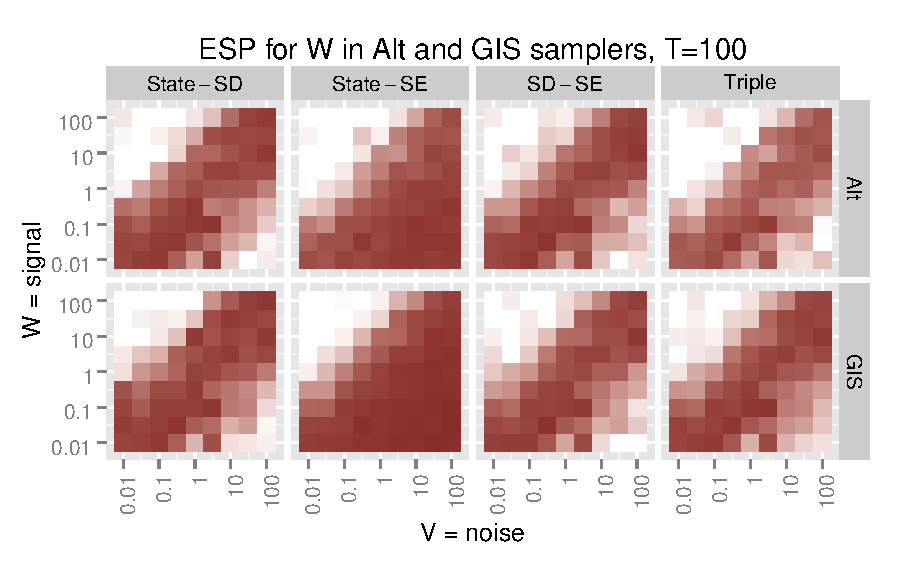
\includegraphics[width=0.45\textwidth]{altintESplotW100}
\end{frame}

\begin{frame}
\frametitle{LLM Results --- ESP for T=1000}
\centering
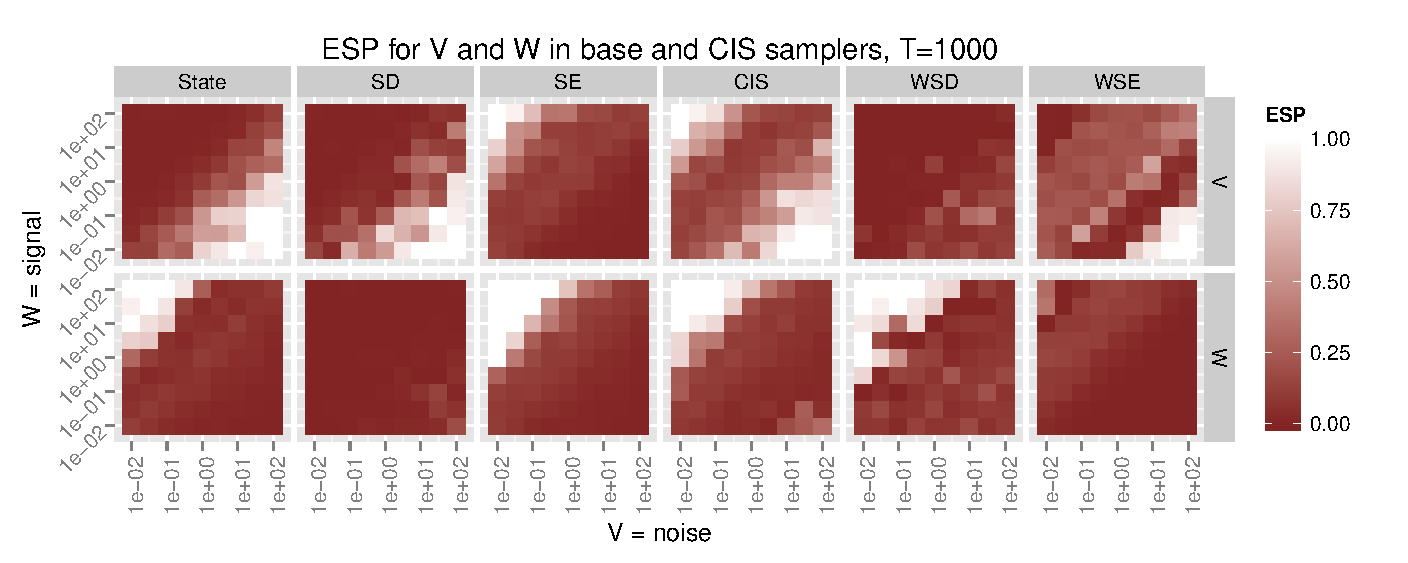
\includegraphics[width=0.59\textwidth]{basecisESplot1000}\\
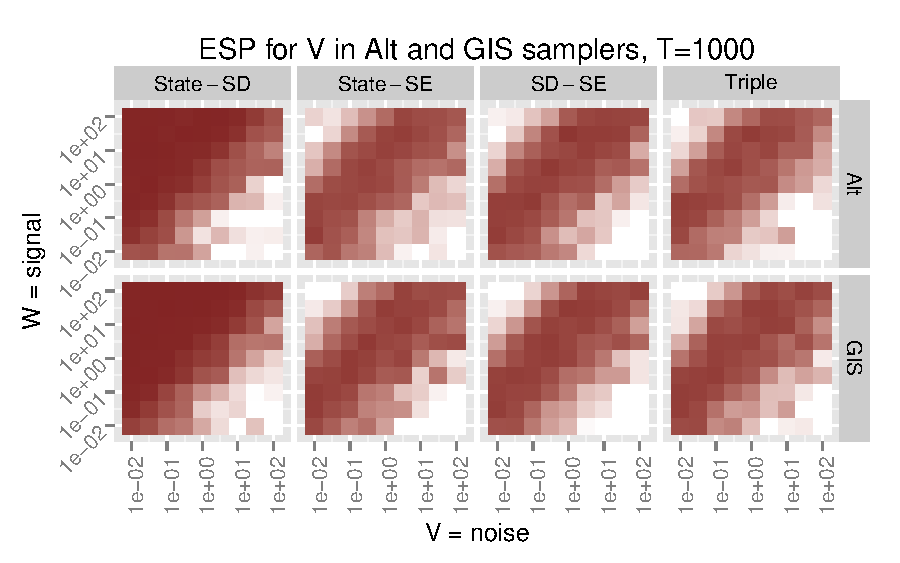
\includegraphics[width=0.53\textwidth]{altintESplotV1000}
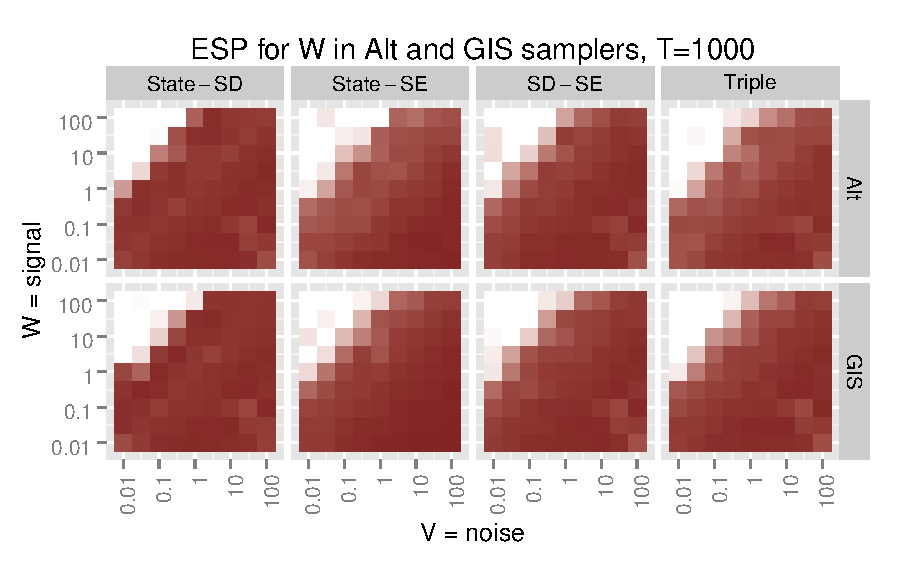
\includegraphics[width=0.45\textwidth]{altintESplotW1000}
\end{frame}

%\begin{frame}
%\frametitle{LLM Results --- ESP summarized}
%Rule of thumb for when each base algorithm has a high ESP for each variable as a function of the true signal-to-noise ratio, $R^*=W^*/V^*$. \\~\\~\\
% \begin{center}
%  \begin{tabular}{lccccc}\hline
%    Parameter & State & SD & SE & WSD & WSE \\\hline
%    V & $R^* < 1$ & $R^* < 1$ & $R^* > 1$ & $R^* < 1$ & $R^* < 1$\\
%    W & $R^* > 1$ & $R^* < 1$ & $R^* > 1$ & $R^* > 1$ & $R^* > 1$ \\
%      &           &          &           &           &           \\\hline
%    Parameter & State-SD        & State-SE       & SD-SE        & Triple            & CIS \\\hline
%    V         & $R^* < 1$           & $R^* \not\approx 1$ & $R^* \not\approx 1$ & $R^* \not\approx 1$ & $R^* \not\approx 1$ \\
%    W         & $R^* \not\approx 1$ & $R^* > 1$           & $R^* \not\approx 1$ & $R^* \not\approx 1$ & $R^* \not\approx 1$\\\hline
%  \end{tabular}\\~\\~\\
%\end{center}
%
%Note that as the length of the time series increases, the farther away from one $R^*$ has to be for the sampler to have a high ESP.
%\end{frame}

\begin{frame}
\frametitle{Moving Forward: Computational Issues}
Major bottleneck: drawing from $p(W|V,\gamma,y)$ and $p(V|W,\psi,y)$:
\begin{align*}
p(x)\propto {\color{blue}x^{-\alpha-1}}\exp[-ax + b\sqrt{x} {\color{blue}- c/x}] 
\end{align*}
What about when $V$ and $W$ are matrices?\\~

$\to$ Need a better prior. E.g. $\pm \sqrt{V} \sim \N(0,\Lambda_V)$\\~\\

Then in the LLM $p(V|W,\theta,y)=p(V|W,\gamma,y)$ is GIG:
\begin{align*}
p(y) \propto y^{\alpha-1}\exp\left[-\frac{1}{2}(ay + b/y)\right] \qquad \alpha\in\Re; a,b,y>0
\end{align*}
What about when $V$ is a matrix?
\end{frame}

\begin{frame}
\frametitle{Moving Forward: Augmenting $F_t$}
Suppose $F_t=\begin{bmatrix}1 & x_t\end{bmatrix}$ and $G_t=1$:
\begin{align*}
y_t &= \begin{bmatrix}1 & x_t\end{bmatrix}\begin{bmatrix}\alpha_t \\ \beta_t\end{bmatrix} + v_t, \qquad v_t\stackrel{iid}{\sim}\N_1(0,V)\\
\begin{bmatrix}\alpha_t \\ \beta_t\end{bmatrix} &= \begin{bmatrix}\alpha_{t-1} \\ \beta_{t-1}\end{bmatrix} + \begin{bmatrix}w_{1,t} \\ w_{2,t}\end{bmatrix}, \qquad \begin{bmatrix}w_{1,t} \\ w_{2,t}\end{bmatrix}\sim\N_2(0,W)
\end{align*}
Easy way to augment the model:
\begin{align*}
\begin{bmatrix}y_t \\ y_t^*\end{bmatrix} &= \begin{bmatrix}1 & x_t\\ 0 & 1\end{bmatrix}\begin{bmatrix}\alpha_t \\ \beta_t\end{bmatrix} + \begin{bmatrix}v_t \\ v_t^* \end{bmatrix}, \qquad \begin{bmatrix} v_t\\ v_t^* \end{bmatrix}\stackrel{iid}{\sim}\N_2\left(0,\begin{bmatrix}V & 0 \\ 0 & 1\end{bmatrix}\right)\\
\begin{bmatrix}\alpha_t \\ \beta_t\end{bmatrix} &= \begin{bmatrix}\alpha_{t-1} \\ \beta_{t-1}\end{bmatrix} + \begin{bmatrix}w_{1,t} \\ w_{2,t}\end{bmatrix}, \qquad \begin{bmatrix}w_{1,t} \\ w_{2,t}\end{bmatrix}\sim\N_2(0,W)
\end{align*}
and add a step to draw $y_{1:T}^*|V,W,\alpha_{1:T},\beta_{1:T},y_{1:T}$.\\~\\

But is this the best way? Or even a good way?
\end{frame}

\begin{frame}[allowframebreaks]
        \frametitle{References}
        \bibliographystyle{plainnat}
        \bibliography{../doc/dlmasis}
\end{frame} 

\end{document}
